\documentclass{article}
\usepackage[utf8]{inputenc}
\usepackage{graphicx}
\usepackage{cite}
\graphicspath{ {./images/} }



\title{Agent-based models of voluntary compliance in non-pharmaceutical interventions for epidemic control}
\author{Robert Brian Milligan and Supervised by Julian Garcia Gallego \& Buser Say}
\date{7 July 2022}


\begin{document}


\maketitle

\begin{abstract}
Epidemic modelling has proven vital for understanding ways in which governments, workplaces and other decisions makers may seek to control the spread of COVID-19. Although many computational models of disease spread exist, not many consider human behaviour explicitly. In this paper, we extend a network-based agent based model to account for ways in which agents can comply or not comply with voluntary non-pharmaceutical interventions. We investigate non-strategic and strategic models of agent compliance and find that the lower the natural reproduction rate of the disease, the higher the chance of achieving success with voluntary non-pharmaceutical interventions. For high R0 values, the best results were found when compliance benefit increase is based on the number of close contacts in an individual has, Whereas for lower R0 values, the best results were found when the benefit for compliance related to looking at the number of agents one was in contact with, that was either symptomatic, hospitalised, fatality or in quarantine. In short, voluntary non-pharmaceutical interventions work best when the natural spread of the disease is relatively slow.
\end{abstract}



\tableofcontents

\newpage 

\section{Introduction}

Mathematical and computational models are important in preparing policies to deal with pandemics. Mathematical models exist ~\cite{cooper_mondal_antonopoulos_2020} that assume an infinite population and place proportions of this population into compartments, traditionally this is SIR, (Susceptible, Infectious and Recovered), however over the years additional have been made, some common examples being SEIR, SIS and SIRV. Computational models use computing power to solve these mathematical models or can be used to apply these concepts to other methods of modelling such as agent based models. These models typically have a finite number of agents which interact with each other in some manner. In regards to epidemiology, these models typically do not incorporate behaviour, or if they do, they do it in simple ways such as compartmental models that incorporate "aggregate states". This means that the model implemented six different behavioural scenarios which would change based on the time of the simulation or having a certain threshold of positive test, positive cases or deaths per day ~\cite{karaivanov_2020}.\linebreak

This paper investigates the modification of an existing model disease spread produced by Ryan McGee and used as a part of various peer reviewed research articles ~\cite{mcgee_homburger_williams_bergstrom_zhou_2021} ~\cite{mcgee_homburger_williams_bergstrom_zhou_2021_2}. 
I have looked at applying this model to the situation of COVID-19 in a childcare setting and involves creating both non strategic and strategic behavioural choice models. \newline

Specifically behaviour in this model relates to compliance to various actions the agent can choose to comply with when requested such as doing a COVID rapid antigen test whenever they have symptoms of the virus. The non strategic model looks at giving agents a fixed cost of complying with requested actions with a reward based on a mix of local situations such as if they are in close contact with an agent who has a symptomatic case of the disease, and a global situation such as the percentage of the group that have reported a positive test within the last 2 weeks. The strategic model looks at agents where they know how all other agents will act and use this information to help them decide if it in their interest to comply.\newline

The rest of this paper is organised as follows. Section 2 describes the basic model. Section 3 describes the childcare scenario and the benchmark model. Section 4 goes though and introduces the Non-Strategic Model. Section 5 goes though the introduces the Strategic Model. Section 6 goes though the results of running the Models. Section 7 discusses the results and future work.


\section{Description of Model \label{description}}
The model that is modified in this paper is an Agent Based Model (ABM). This ABM is one where agents can belong to one and only one compartment representing their state. 

Agents progress though states with the only sink node being Recovered and Fatality
the states of Susceptible, Exposed, Pre-Infectious, Infectious-Asymptomatic, Infectious-Symptomatic, Hospitalised, Fatality and Recovered exist. All these except Hospitalised and Fatality can have agents in a mirror state where they are also isolated, meaning they cannot acquire the disease or spread it to any other agents in the network.

Once an agent catches the disease they move along the stages of the disease until they are a fatality or recovered, at any point they have the ability to move across to the mirror isolation state. 



\begin{figure}
\centering
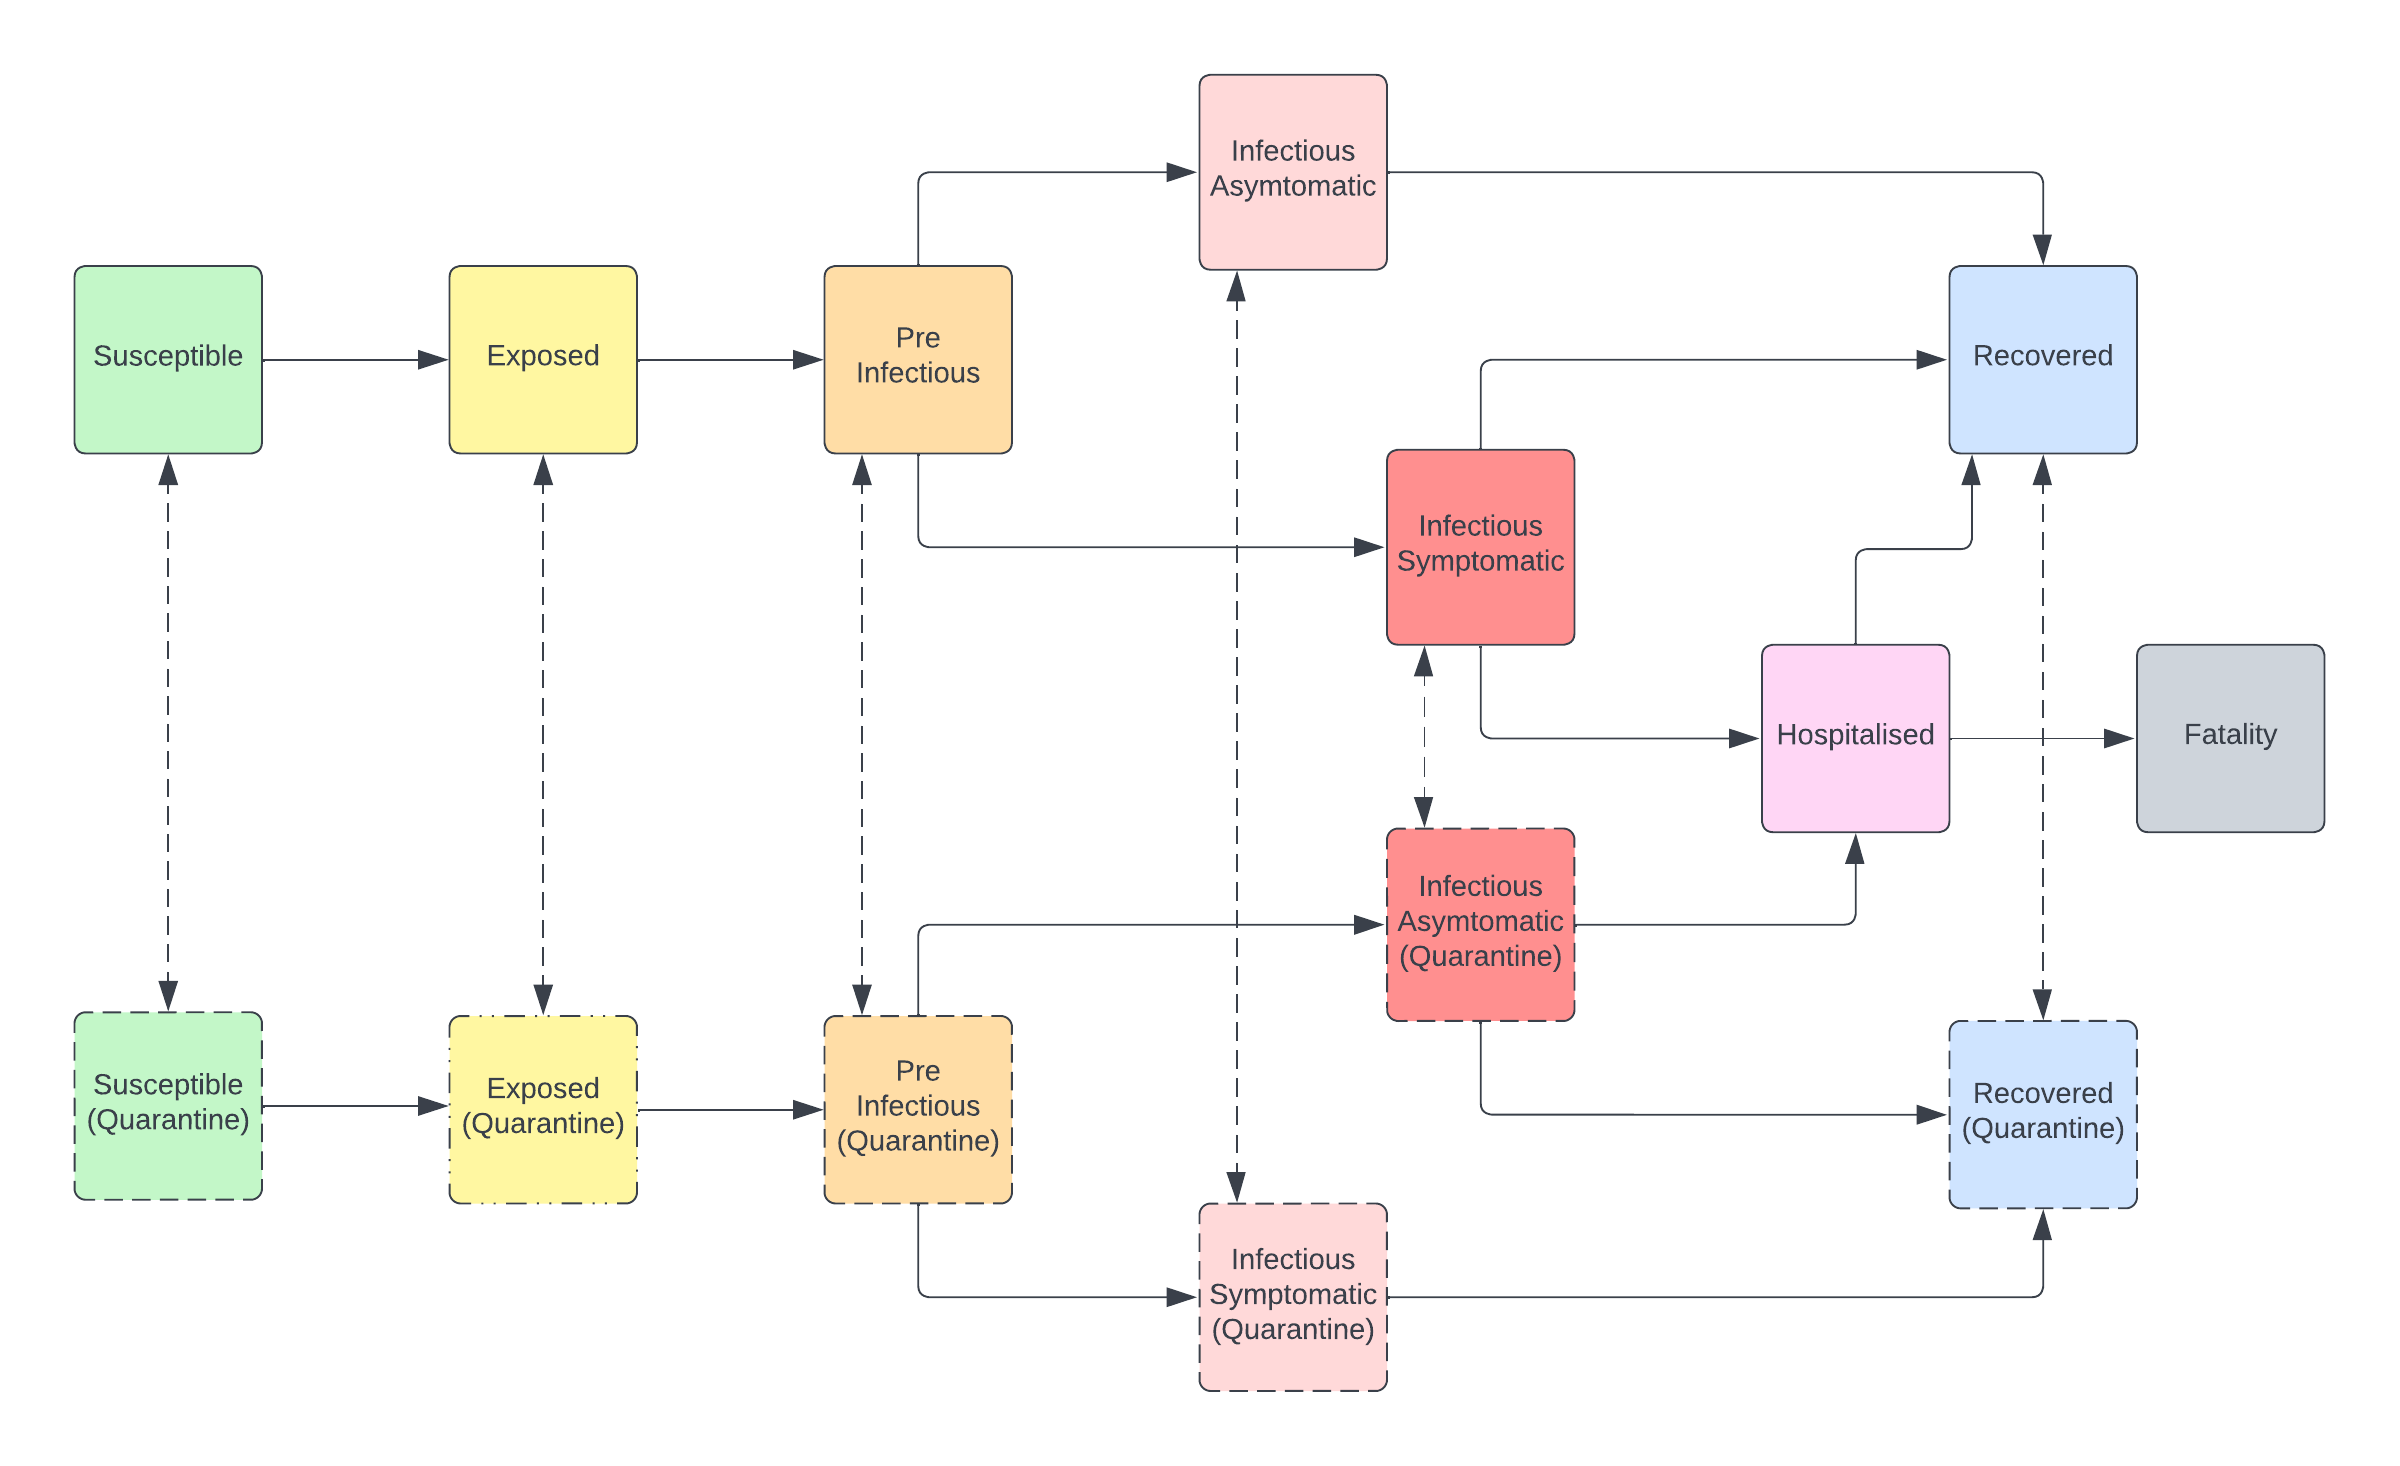
\includegraphics[width=\textwidth]{SIR}
\caption{a diagram of the existing model of seirplus ~\cite{mcgee_2021}}
\end{figure}

\newpage



\subsection{Using networks to model contacts}

The version of the model we use considers a simple network, one which uses a one single connected network designed to simulate a workplace.

These large networks are made up of a number of cohorts which are loosely connected and each of these cohorts can have a number of subgroups which are highly connected.

The network is set up before the simulation begins and is different every time and does not change throughout the simulations run. 

Agents are arranged in a network as nodes and are connected by edges representing which other nodes are their close contacts. 80\% of disease spread is though the close contact edges and 20\% is spread randomly.

\subsection{Compliance in the model}
Each day agents will be asked to do a test if their day has come up on a surveillance testing schedule, they show symptoms or have been contacted that they are a close contact. However there is a compliance value to them following through with the requested action

During the day agents can spread the contagion to each other and can progress though the stages of the disease if they have it. They additionally have the choice to participate in contact tracing.

Agents will also be asked to isolate for one of six reasons. They or a group member develop a symptomatic case, returns a positive test or is told they are a close contact though using contact tracing. Again there is a compliance value to decide if they follow through with the requested action

These systems can effectively be disabled by overriding the compliance for them to be a large negative number, for example compliance with contact tracing can be set to -10 to disable the use of that system and this done to limit the model to a smaller number of variables which compliance can affect.

The Current Modifications of the model relate to allowing 10 of the Model Parameters that relate to Compliance to be dynamically updated each day dependent on a given rule. Those that we use in this paper and dynamically change are the testing if the agent develops a symptomatic case as well as surveillance testing 

Compliance can be set a variety of ways in the modified model.
\begin{itemize}
\item The default setting where agents are given an initial value for compliance and is unchanging e.g. 50\% are set to comply and will always do so
\item The non strategic model where agents are given an initial compliance and can become more compliant depending on the network situation , their local situation or a mix
\item The strategic model where agents utilise knowledge of the amount of agents in the network who will comply to make a decision to comply or not
\end{itemize}

Lastly, the model has a variety of limitations including 
\begin{itemize}
\item Having all agents always test on the same day, thus if semi-weekly is chosen, all agents will be asked to test on Monday and Thursday
\item the network itself is unchanging, however this is not necessarily bad as it removes a variable that may change results
\end{itemize}

\newpage



\newpage
\section{Childcare Scenario and Benchmark Baseline Model}


A childcare scenario was chosen for a few reasons, among them are that the model works best with networks of a relatively small size of less than 200 agents, the network structure of the model could be used to reflect the dynamics that would be apparent in a child care building and parameters could be chosen to match this specific scenario.\newline

Parameter justification

\begin{table}[h!]
\begin{tabular}{ll}
Test False negative rate & 0.36 ~\cite{van_de_mortel_2022} \\
R0 mean of Omicron is 9.5 and Delta is 5.4 & ~\cite{liu_rocklov_2022} \\
Isolation as a result of a Positive Test & 100\%
\end{tabular}
\end{table}

\begin{figure}[h!]
\centering
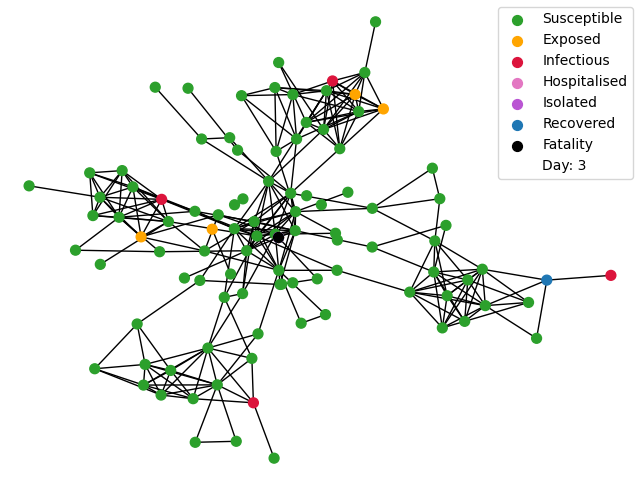
\includegraphics[width=\textwidth]{network}
\caption{An Example Network}
\end{figure}

This is an example of the network of 100 agents
To simulate the childcare scenario they are split into 5 groups of about 20 agents each with high connectivity inside the group and low connectivity between the groups 
The agents current state is shown by the nodes colour and the edges are that agents close contacts which the disease can spread easiest though the population\newline

For the benchmark baseline runs compliance for behaviour is set at levels of 0.5 and 1, to represent 50\% of agents and all agents complying. If agents are compliant, they will perform symptomatic test and regular interval surveillance tests when asked.\newline

The R0 (The disease basic replication rate) of 9.5 or 5.4 may be too high as it assumes children spread the disease at the same rate as the general population as well as all disease spread of children occurring in entirely in the childcare location which is probably not the case. Therefore two other R0 cases of 3 and 2 are used as they may more accurately capture a real world scenario where not all transmission is though the childcare setting.\newline

\begin{figure}
\centering
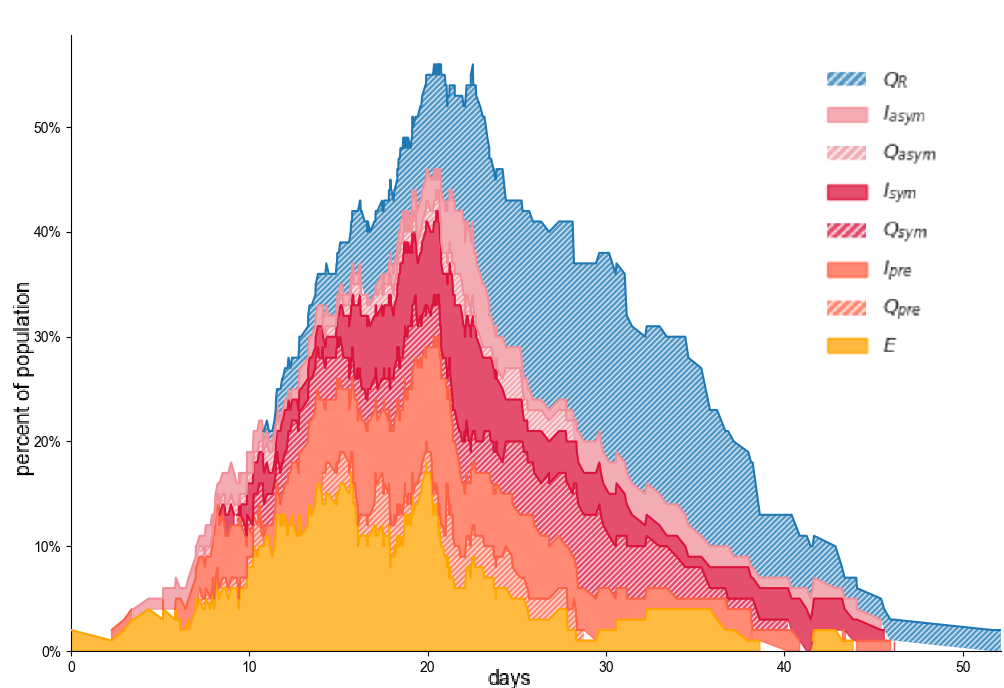
\includegraphics[width=\textwidth]{Figure3}
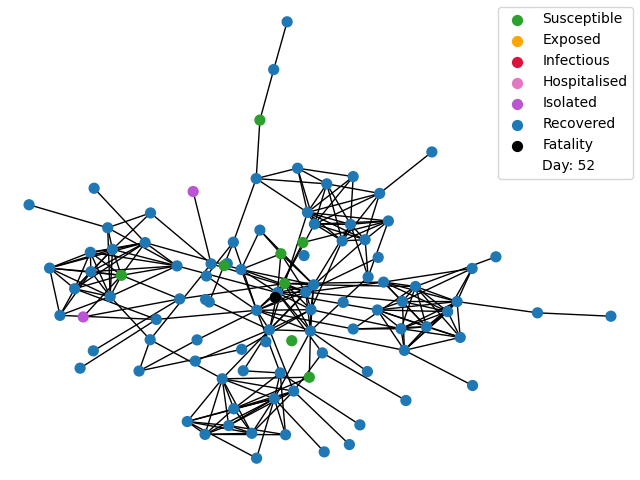
\includegraphics[width=\textwidth]{Figure3Net}
\caption{Benchmark Run with Unchanging Compliance at 50\% for regular twice weekly surveillance testing and testing if symptomatic with the resulting final network. 92 of the 100 agents received the infection}
\end{figure}


The benchmark model is associated with one single large peak of disease spread

There are 5 models compared these are
Baseline 50\% compliance, this is where each agent when generated has a 50\% chance to always or to never comply. 

Baseline 100\% compliance, this is where each agent when generated has a 100\% chance to always comply. 

\newpage

\section{Non-Strategic Model}
With the non-strategic model we have a fixed cost of compliance and can have varying factors that can raise it. A mix of global and local behavioural factors can be added to make an agent more compliant. In the current build these are the known positive cases in the network in the past 14 days. The proportion of contact agents (those which share an edge) which are a fatality, hospitalised or in isolation. These values are taken away from the base cost and if the result is lower from a specified value the agent will be compliant to that action, otherwise they are not

For a simple example we have a situation for this central agent 

\begin{figure}[h!]
\centering
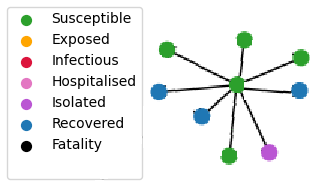
\includegraphics[width =150pt]{basicnet}
\caption{An Example Simplified Network}
\end{figure}


\begin{table}[h!]
\begin{tabular}{ll}
Symptomatic Testing Rate Compliance & 50\% \\
Surveillance Testing Rate Compliance & 50\% \\
This agent’s base aptitude & uniformly distributed (-0.1,0.1) \\
Base Cost of Compliance & 0.5 
\end{tabular}
\end{table}

Compliance = 0.5 – (5 * 1/8) – (5*0.02) + 0.1 = -0.105

In this case the agent is compliant

for the non-strategic model to give the agents diversity, initially a value is generated that is used in all compliance calculations for them that either biases them to be more or less compliant, for example the base attitude for an agent might be 0.1; meaning the benefit would have to be 0.1 greater than that of a completely neutral agent for them to comply.\newline

This model is used for one case where the fixed cost is set at 0.5, we call this Non-Strategic Minimum 50\% , and is where each day the compliance value for an agent is updated and changes based on a combination of the global known positive test cases recorded in the network within the last 14 days as well as the proportion of close contacts of an agent that are either symptomatic, a fatality, hospitalised or in isolation.\newline


\section{Strategic Model}
The view of benefit and cost can be grouped into 3 categories.
There is a level at which people will not contribute as they find the act pointless as they know near no agents will comply 

For the strategic model a curve is created to model a game theory dilemma on wherever or not the agent should comply given they know the cost and reward for compliance and what every other agent will do, depending on the benefit the likelihood of any one agent complying can vary from 0, to 60-99\% to 100\%.

This model is used in three cases and is designed like the non-strategic model to have a baseline of 50\% compliance which grows based on the following rules:\newline

Strategic Community Size, this is where the benefit to compliance is based on the number of close contacts the agent has. This is a case where the curve is different for each agent but unchanging over time.\newline\newline
Strategic Local State, this is where the benefit to compliance is based on the number of close contacts that are either in a state of symptomatic, a fatality, hospitalised or in isolation. This is a case where the curve is different for each agent and unchanging over time.\newline\newline
Strategic Global State, this is where the benefit to compliance is based on the number of agents in the network that are either in a state of symptomatic, a fatality, hospitalised or in isolation. This is a case where the curve is the same for each agent but changes over time.

\section{Results}

To evaluate the result of the model, those of the baseline, non-strategic and strategic we look at two key parameters, the percentage of agents that contracted the disease and the number of days that elapsed until zero agents were infectious.\newline

In this model two choices of compliance are considered, If an agent is compliant they will perform semi-weekly surveillance testing in addition to testing whenever they develop a symptomatic case of the disease, If they are not compliant they will do neither of these actions.\newline


\begin{figure}[h!]
\centering
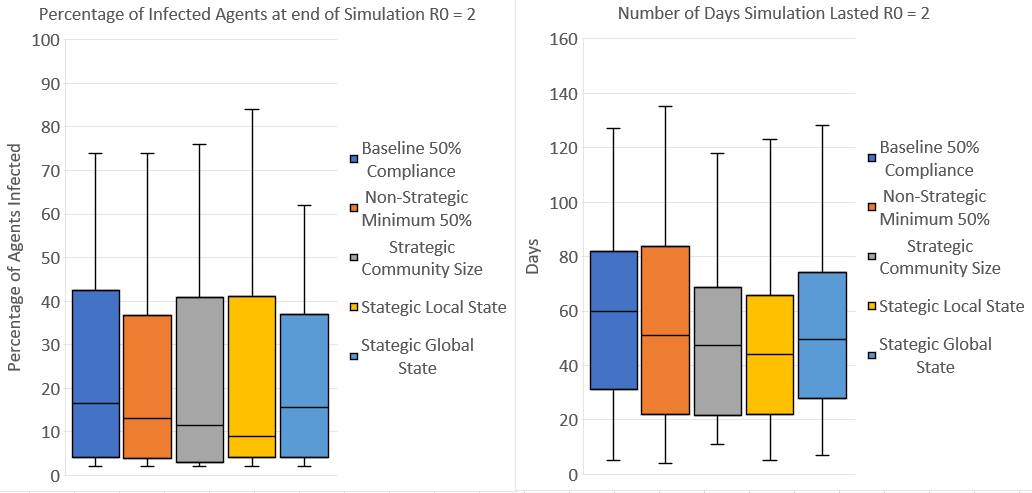
\includegraphics[width=\textwidth]{5}
\caption{Test Results over R0 of 2}
\end{figure}

\newpage
\begin{figure}[h!]
\centering
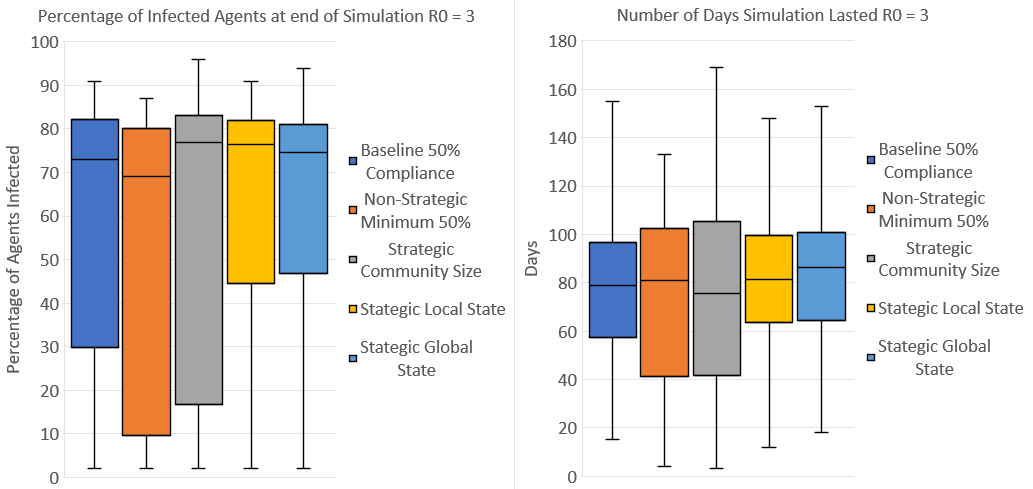
\includegraphics[width=\textwidth]{4}
\caption{Test Results over R0 of 3}
\end{figure}

\begin{figure}[h!]
\centering
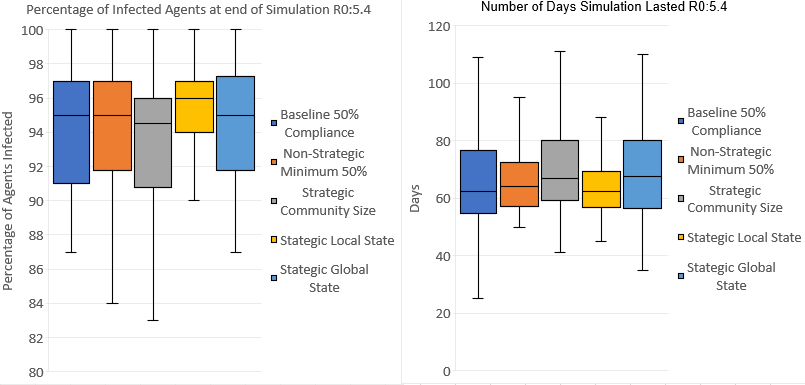
\includegraphics[width=\textwidth]{3}
\caption{Test Results over R0 of 5.4}
\end{figure}
\newpage
\begin{figure}[h!]
\centering
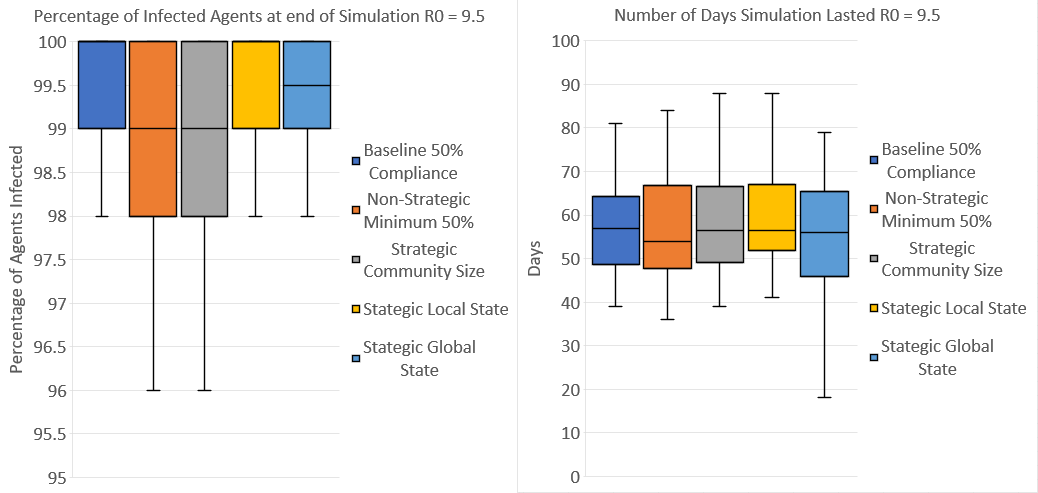
\includegraphics[width=\textwidth]{2}
\caption{Test Results over R0 of 9.5}
\end{figure}

\begin{figure}[h!]
\centering
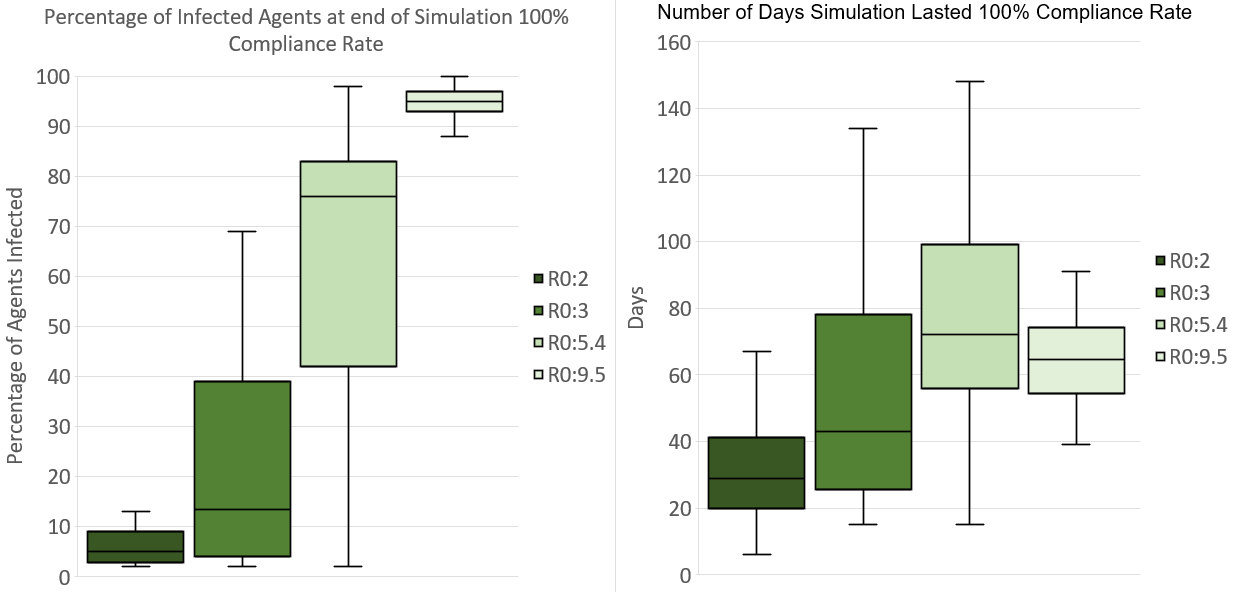
\includegraphics[width=\textwidth]{6}
\caption{Test Results over all R0 values at 100\% Compliance}
\end{figure}


\begin{figure}[h!]
\centering
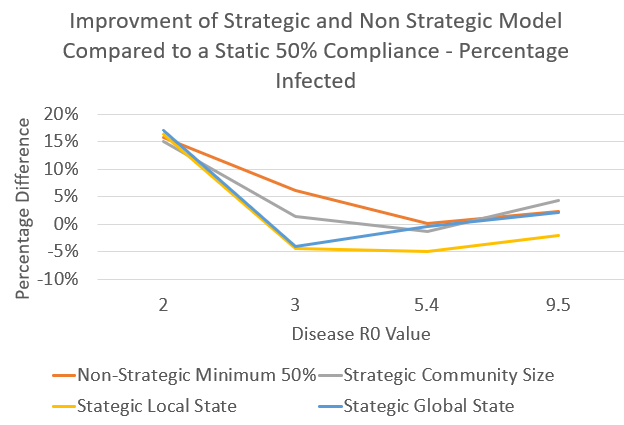
\includegraphics[width=\textwidth]{1}
\caption{Test Results Comparing the Results of R0 values}
\end{figure}
\newpage


\section{Discussion}

\subsection{Analysis of Percentage of Infected Agents}

Over 4 different R0 virus base reproduction rate numbers the model was run with, for those apart from the 100\% compliance baseline saw a reduction in total cases from a -2\% improvement with an R0 of 9.5 to a 17\% improvement with an R0 of 2. This is probably a result of agents having more time to choose to be compliant, as the disease spreads slower though the system and already compliant agents have a chance to go though a run of surveillance testing and potentially isolate before they have infected many other individuals. With extremely high R0 numbers it is observed that the non-strategic and strategic behavioural model have little effect on the total number infected. Across all cases it can be seen that the amount of time the simulation runs for is tied with how many agents get infected. Both the static values of compliance and non-strategic behavioural model follow this trend.\newline 

The non-strategic model was found to be the most effective in reducing the number of infected agents throughout the R0 values of 3 and 5.4 but by 9.5, the strategic community size model was found to be more effective. This could be a result of the non-strategic model taking into account both the global spread of the disease in the network as well as the current compartment / state of close contacts impacting compliance. In the case of extremely high R0 values the strategic community size model which only considers the number of close contacts an agent has when considering if there are to be compliant or not had the greatest improvement, this could be the case as forces those most central agents to be compliant and therefore are not able to spread the disease far across the network, forcing it to stay more localised where it has the opportunity to die out before it becomes an epidemic in the network.\newline 

\subsection{Analysis of Time Disease Took to Stop spreading}

Regarding the days the simulation took before disease spread stopped, it was found that the strategic models particularly at the lower R0 values of 2 and 3 saw significant improvement. This is interesting as while similar percentages of agents were infected, the time it took for the disease to die out was less, suggesting the disease spread through the network faster but ultimately had about the same proportion of agents who ended up getting the disease.\newline 

Notably the case of Strategic Local State where agents use the number of agents around them who are in a high risk state to decide if they are compliant fared the worst at a disease R0 value of 9.5 having a 2\% increase in infected agents and it taking 6\% longer for the disease to stop spreading, this would suggest that agents who base decisions about if to test based solely on how their close contacts are faring is not a good approach at reducing the spread of disease and more global measures or measures that rely on how central a person is in their network of close contacts are more effective. \newline 

future work .....


\newpage
\appendix

\section{Appendix Section}
The code for the modified version of the model is located here https://github.com/robertmxmx/seirsplus-dynamic-agents
The confrence style used is that of AAMAS (International Conference on Autonomous Agents and Multiagent Systems) 


\bibliography{bibliography}{}
\bibliographystyle{plain}

\end{document}


\end{document}

